\documentclass[11pt]{scrartcl}
\usepackage[sexy]{evan}
\usepackage{graphicx}
\usepackage[spanish]{babel}
\graphicspath{ {./images/} }

\usepackage{answers}
\Newassociation{hint}{hintitem}{all-hints}
\renewcommand{\solutionextension}{out}
\renewenvironment{hintitem}[1]{\item[\bfseries #1.]}{}

\usepackage{venndiagram,multicol,hyperref,graphicx,array}

\begin{document}
\title{Tableros}
\author{Ricardo Largaespada}
\date{04 Mayo 2024}

\maketitle
\section{Introducción}
¿Quien nunca jugó al rompecabezas? Tenemos varias ``piezas'' y tenemos que encontrar una manera de unirlas todas para formar una figura más grande. Lo que solía ser solo un pasatiempo, ganó una hermana que fue estudiada por muchos matemáticos serios en todo el mundo: la ``Tiling Theory'' (traducida como: Teoría del Recubrimiento). Y debido a ser un tema muy atractivo, rápidamente ganó fuerza en las principales competiciones de matemáticas.

\begin{example}
Determine si es posible cubrir o no el tablero a continuación (sin superposiciones) usando solo dominós.
\begin{center}
    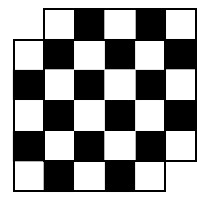
\includegraphics[width=4cm]{images/clase_combi_centro_09_chess_board_no_coners.png}
\end{center}
\end{example}
Solución. Pinte las casillas del tablero alternativamente de blanco y negro (como en el tablero de ajedrez). Note que, no importa cómo coloquemos el dominó en el tablero, siempre cubrirá una casilla blanca y otra negra. Por lo tanto, si fuera posible cubrir el tablero usando solo dominós, deberíamos tener la misma cantidad de casillas negras que de casillas blancas. Pero en el tablero ``roto'' hay 18 casillas blancas y 16 negras. Por lo tanto, no es posible hacer tal cobertura.

\begin{example}
    ¿Podemos cubrir un tablero 10 $\times$ 10 usando solo T-tetraminós como se muestra a continuación?
    \begin{center}
        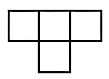
\includegraphics[width=2cm]{images/clase_combi_centro_09_title.png}
    \end{center}
\end{example}
Solución. Pinte el tablero de blanco y negro de manera habitual (como en el ajedrez). Note que al colocar un T-tetraminó en el tablero, puede tener colores del tipo 1 o 2.
\begin{center}
    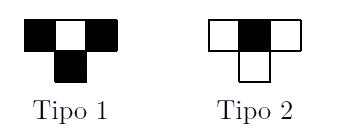
\includegraphics[width=4cm]{images/clase_combi_centro_09_title_solucion.png}
\end{center}
Suponga que al cubrir el tablero usamos A piezas del tipo 1 y B del tipo 2. Sabemos que debemos usar 25 piezas en total, es decir, $A + B = 25$. Cada pieza del tipo 1 ocupa una casilla blanca y cada pieza del tipo 2 ocupa 3 casillas blancas, y como hay un total de 50 casillas blancas en el tablero; $A + 3B = 50$. De manera análoga, obtenemos $B + 3A = 50$. Sin embargo, el sistema anterior no tiene solución entera. Por lo tanto, no es posible cubrir el tablero.\\

Y no es solo el coloreo como tablero de ajedrez es lo que es útil para resolver problemas. Veamos el siguiente ejemplo.

\begin{example}
    ¿Para qué valores de \(n, m\) podemos cubrir un tablero \(n \times m\) usando solo L-tetraminós como se muestra a continuación?
    \begin{center}
        
\includegraphics[width=2cm]{images/clase_combi_centro_09_ele.png}
    \end{center}
\end{example}
Solución. Claramente, $n \times m$ debe ser un múltiplo de 4. En este caso, \(n\) o \(m\) (posiblemente ambos) deben ser múltiplos de dos. Supongamos sin pérdida de generalidad que $m$ (es decir, el número de columnas) es par. Pinte alternativamente las columnas de dos colores como se muestra en la figura anterior. Para finalizar, adapte la solución del problema anterior.

\begin{figure}[h]
    \centering
    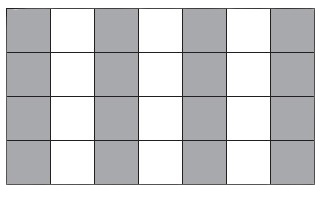
\includegraphics[width=4cm]{images/clase_combi_centro_09_ele_solucion.png}
    \caption{Coloreo por columnas.}
\end{figure}

Si dos colores ayudan a mucha gente, ¡cuatro colores ayudan mucho más! ¡Es cierto! No pienses que solo pintando el tablero de negro y blanco resolverás todos los problemas de tablero del mundo. El siguiente ejemplo muestra que a veces solo dos colores no son suficientes.

\begin{example}
    ¿Es posible que un caballo de ajedrez pase por todas las casillas de un tablero 4 $\times$ 10 exactamente una vez y luego regrese al cuadrado original?
\end{example}
    \begin{center}
        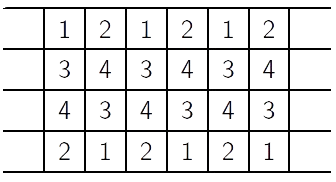
\includegraphics[width=4cm]{images/clase_combi_centro_09_problema_4.png}
    \end{center}
Solución. Pinte el tablero $4 \times n$ como se muestra en la figura anterior. Suponga que es posible que el caballo pase por todas las casillas. Note que si el caballo está en la casilla 1 solo puede ir a la casilla 3; de esta manera, para que el caballo vaya a una casilla de color 1, pasa por dos casillas de color 3, y como cada color tiene el mismo número de casillas, es imposible que el caballo haga el recorrido.\\

Vimos que pintar tableros usando colores es una excelente idea. ¡Una idea aún mejor es pintar usando números! Debe estar preguntándose ¿por qué? Bueno, los números tienen propiedades aritméticas (es decir, se pueden sumar y multiplicar), algo que no podemos hacer con colores. A menos que pienses que negro + blanco = gris.

\begin{example}[Estonia 1993]
    ¿Para qué naturales \(n\) no es posible cubrir un rectángulo de tamaño $3 \times n$ con las piezas mostradas en la figura sin superposiciones?
\begin{center}
    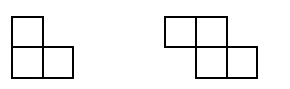
\includegraphics[width=4cm]{images/clase_combi_centro_09_problema_5.png}
\end{center}
\end{example}
Solución. Pinte el tablero de la siguiente manera:

\begin{center}
    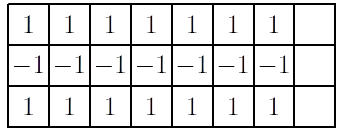
\includegraphics[width=4cm]{images/clase_combi_centro_09_problema_5_solucion.png}
\end{center}

Observe que la suma de los números cubiertos por un L-trinomino es siempre $1$ o $-1$, mientras que la suma de los números cubiertos por un Z-tetramino es siempre cero. Además, la suma de todos los números del tablero es \(n\). Observe que para cubrir un tablero $3 \times n$ podemos usar como máximo \(n\) piezas.\\

Por lo tanto, todas las piezas deben ser L-trinominos. Además, no podemos colocar ningún L-trinomino de modo que la suma de los números escritos en sus casillas sea $-1$. Por lo tanto, si pintamos el tablero como en el ajedrez, cada L-trinomino tendrá que ocupar dos casillas negras. Por lo tanto, \(n\) debe ser un número par.

\Opensolutionfile{all-hints}

\section{Problemas Propuestos}

\begin{problem}
Encuentra el menor lado de un tablero cuadrado que puede ser ensamblado usando el mismo número de piezas de cada uno de los siguientes tipos.
\begin{center}
    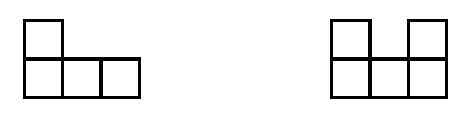
\includegraphics[width=4cm]{images/clase_09_L_y_U_tetramino.png}
\end{center}
\end{problem}

\begin{problem}
Sobre una de las casillas de un tablero infinito, hay un cubo que cubre perfectamente la casilla. La cara en la parte superior del cubo es blanca, mientras que las demás caras son negras. En cada paso, podemos voltear el cubo hacia uno de los lados. ¿Es posible que:\begin{itemize}
\item[(a)] Después de 2004 pasos el cubo vuelva al mismo cuadrado con la cara blanca hacia abajo?
\item[(b)] Después de 2005 pasos?
\end{itemize}
\end{problem}

\begin{problem}
¿Es posible cubrir el siguiente tablero usando solo dominós?
\begin{center}
    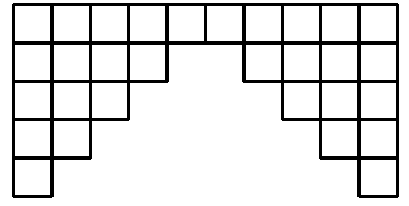
\includegraphics[width=4cm]{images/clase_09_problema_dominos.png}
\end{center}
\end{problem}

\begin{problem}
¿Es posible cubrir un tablero $5 \times 10$ usando solo piezas como se muestra a continuación?
\begin{center}
    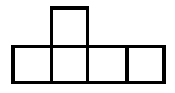
\includegraphics[width=2cm]{images/clase_09_problema_quintimino.png}
\end{center}
\end{problem}

\begin{problem}
 Queremos cubrir un tablero $7 \times 7$ usando varias piezas de dos tipos:
\begin{center}
    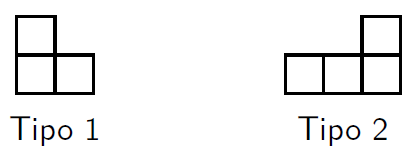
\includegraphics[width=4cm]{images/clase_combi_centro_09_L_trimino_y_L.png}
\end{center}
Indique cómo cubrir el tablero usando el menor número posible de piezas del tipo 1.
\end{problem}

\begin{problem}[Rusia 1997]¿Podemos cubrir un tablero $75 \times 75$ usando dominós y cruces?
\begin{center}
    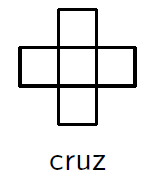
\includegraphics[width=2cm]{images/clase_09_cruz.png}
\end{center}
\end{problem}

\begin{problem}[Rioplatense 1999] ¿Es posible cubrir un tablero $1999 \times 1999$ con cuadrados de lados enteros mayores que 35 y menores que 1999.
\end{problem}

\begin{problem}[Rusia 2007] Las caras de un cubo $9 \times 9 \times 9$ están divididas en cuadritos de la forma habitual. Su superficie está cubierta por 243 tiras de papel $2 \times 1$ sin superposición. Una tira se considera doblada si no está solo sobre una cara. Demuestre que el número de tiras dobladas es impar.
\end{problem}

\begin{problem}
¿Podemos cubrir una caja $10 \times 10 \times 10$ con 250 cajas $1 \times 1 \times 4$?
\end{problem}

\begin{problem}
Un tablero $n \times m$ fue completamente cubierto usando piezas $4 \times 1$ y $2 \times 2$. Luego, todas las piezas fueron retiradas del tablero y una pieza $2 \times 2$ fue reemplazada por una pieza $4 \times 1$. Demuestra que el tablero no puede ser cubierto nuevamente con este cambio.
\end{problem}

\begin{problem}
De un tablero $n \times n$ se eliminan sus cuatro esquinas. ¿Cuáles son los valores de $n$ para los cuales este tablero roto es cubierto por L-tetraminós?
\end{problem}

\begin{problem}
Sean $m$ y $n$ enteros mayores que 1. Si un tablero $m \times n$ puede ser cubierto con L-tetraminós, entonces $mn$ es múltiplo de 8.
\end{problem}

\begin{problem}[Teorema de Klarner] Un tablero $a \times b$ puede ser cubierto usando solo piezas $1 \times n$ si y solo si $n | a$ o $n | b$.
\end{problem}

\begin{problem}[Rumanía 2000] Determine todos los tableros $m \times n$ que pueden ser cubiertos usando L-triminós como se muestra a continuación:
\begin{center}
    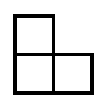
\includegraphics[width=2cm]{images/clase_09_L_trimino.png}
\end{center}
\end{problem}

\begin{problem}
Un tablero $7 \times 7$ está cubierto usando 16 piezas $3 \times 1$ y un monomino. Determine todas las posiciones posibles del monomino.
\end{problem}

\begin{problem}[Estonia 2004] Un tablero $5 \times 5$ está cubierto por ocho L-triminós y un monomino. Determine todas las posiciones posibles que puede ocupar el monomino.
\end{problem}

\begin{problem}
¿Cuál es el número máximo de S-tetraminós como se muestra a continuación que se pueden colocar, sin superposición, en un tablero $10 \times 10$?
\begin{center}
    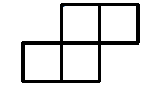
\includegraphics[width=2cm]{images/clase_09_S-tetramino.png}
\end{center}
\end{problem}

\begin{problem}
Un tablero \(7 \times 7\) ´es cubierto usando piezas del siguiente tipo:
\begin{center}
    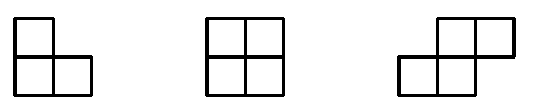
\includegraphics[width=4cm]{images/clase_combi_centro_09_triminos_tetramino.png}
\end{center}
Demuestra que sólo se utiliza una pieza con cuatro casillas.
\end{problem}

\begin{problem}[Bielorrusia 1999] Tenemos un tablero $7 \times 7$ y piezas de los tres tipos siguientes:
\begin{center}
    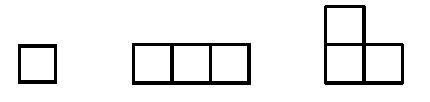
\includegraphics[width=4cm]{images/clase_combi_centro_09_triminos_mono.png}
\end{center}
Samuel tiene infinitas piezas del tipo 2 y una pieza del tipo 3, mientras que Marcelo solo tiene una pieza del tipo 1.
\begin{enumerate}
    \item Demuestra que Marcelo puede colocar su pieza en algún lugar del tablero de manera que Samuel no pueda completar el resto del tablero usando sus piezas.
    \item Suponga que Samuel adquirió otra pieza del tipo 3.
\end{enumerate}
Demuestra que no importa el lugar en el que Marcelo coloque su pieza, Samuel siempre podrá completar el tablero.
\end{problem}

\begin{problem}[IMO 2004] Un gancho es una figura de seis casillas como se muestra en la figura o cualquiera de las figuras obtenidas de esta aplicando rotaciones o reflexiones. Determine todos los tableros $m \times n$ que pueden ser cubiertos usando estos ganchos.
\begin{center}
    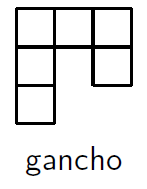
\includegraphics[width=2cm]{images/clase_09_gancho.png}
\end{center}
\end{problem}

\begin{problem}[Putnam 1991] ¿Existe algún número natural $L$, tal que si $m$ y $n$ son enteros mayores que $L$, entonces todo tablero $m \times n$ puede ser cubierto usando piezas $4 \times 6$ y $5 \times 7$?
\end{problem}

\begin{problem}[Bielorrusia 2000] Encuentra el mayor número de cruces que pueden cubrir un tablero $8 \times 8$.
\end{problem}

\begin{problem}[Bielorrusia 2000] Encuentra el mayor número de T-hexaminós (como se muestra a continuación) que pueden cubrir un tablero $9 \times 9$.
\begin{center}
    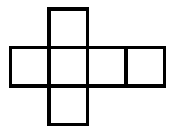
\includegraphics[width=2cm]{images/clase_09_hexamino.png}
\end{center}
\end{problem}

\begin{problem}[Estonia 2004] Encuentra la medida del lado del cubo más pequeño que puede ser cubierto por crymbles.
\begin{center}
    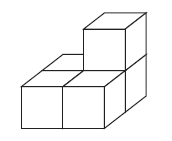
\includegraphics[width=2cm]{images/clase_09_crymble.png}
\end{center}
\end{problem}

\begin{problem}[Rusia 1996] ¿Podemos cubrir un tablero $5 \times 7$ con L-triminós de manera que cada casilla del tablero sea cubierta por el mismo número de piezas?
\end{problem}

\begin{problem}
Supongamos que 99 piezas de $2 \times 2$ se colocan en un tablero $29 \times 29$. Demuestra que todavía se puede colocar otra pieza.
\end{problem}

\begin{problem}
Determine si la última pieza de un juego de resta uno puede terminar en la casilla indicada.
\begin{center}
    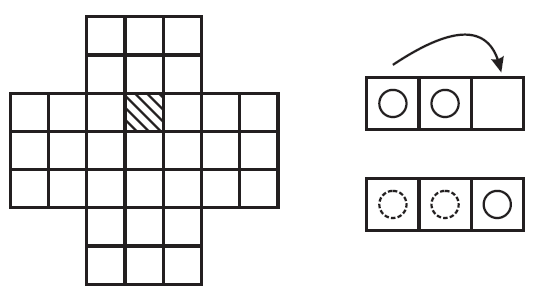
\includegraphics[width=4cm]{images/clase_09_Resta_Um.png}
\end{center}
\end{problem}

\Closesolutionfile{all-hints}

%\section{Sugerencias y Soluciones}
%\begin{enumerate}
%\input{all-hints.out}
%\end{enumerate}

\end{document}